\section{無限時間最適フィードバック制御モデル}
\subsection{モデルの構造}
\textbf{無限時間最適フィードバック制御モデル}\index{むげんじかんさいてきふぃーどばっくせいぎょもでる@無限時間最適フィードバック制御モデル} (\textbf{infinite-horizon optimal feedback control model}\index{infinite-horizon optimal feedback control model}) \cite{Qian2013-zy}


\begin{align}
d x&=(\mathbf{A} x+\mathbf{B} u) dt +\mathbf{Y} u d \gamma+\mathbf{G} d \omega \\
d y&=\mathbf{C} x dt+\mathbf{D} d \xi\\
d \hat{x}&=(\mathbf{A} \hat{x}+\mathbf{B} u) dt+\mathbf{K}(dy-\mathbf{C} \hat{x} dt)
\end{align}
\subsection{実装}
ライブラリの読み込みと関数の定義.
\lstinputlisting[language=julia]{./text/motor-learning/infinite-horizon-ofc/002.jl}
定数の定義


\begin{align}
\alpha_{1}&=\frac{b}{t_{a} t_{e} I},\quad \alpha_{2}=\frac{1}{t_{a} t_{e}}+\left(\frac{1}{t_{a}}+\frac{1}{t_{e}}\right) \frac{b}{I} \\
\alpha_{3}&=\frac{b}{I}+\frac{1}{t_{a}}+\frac{1}{t_{e}},\quad b_{u}=\frac{1}{t_{a} t_{e} I}
\end{align}
\lstinputlisting[language=julia]{./text/motor-learning/infinite-horizon-ofc/004.jl}

\begin{align}
\mathbf{X}\triangleq\begin{bmatrix}
x \\
\tilde{x}
\end{bmatrix}, d \bar{\omega} \triangleq\begin{bmatrix}
d \omega \\
d \xi
\end{bmatrix}, \bar{\mathbf{A}} \triangleq\begin{bmatrix}
\mathbf{A}-\mathbf{B} \mathbf{L} & \mathbf{B} \mathbf{L} \\
\mathbf{0} & \mathbf{A}-\mathbf{K} \mathbf{C}
\end{bmatrix}\\
\bar{\mathbf{Y}} \triangleq\begin{bmatrix}
-\mathbf{Y} \mathbf{L} & \mathbf{Y} \mathbf{L} \\
-\mathbf{Y} \mathbf{L} & \mathbf{Y} \mathbf{L}
\end{bmatrix}, \bar{G} \triangleq\begin{bmatrix}
\mathbf{G} & \mathbf{0} \\
\mathbf{G} & -\mathbf{K} \mathbf{D}
\end{bmatrix}
\end{align}


とする.元論文では$F, \bar{F}$が定義されていたが,$F=0$とするため,以後の式から削除した.


\begin{align}
\mathbf{P} &\triangleq\begin{bmatrix}
\mathbf{P}_{11} & \mathbf{P}_{12} \\
\mathbf{P}_{12} & \mathbf{P}_{22}
\end{bmatrix} = \mathbb{E}\left[\mathbf{X} \mathbf{X}^\top\right] \\
\mathbf{V} &\triangleq\begin{bmatrix}
\mathbf{Q}+\mathbf{L}^\top R \mathbf{L} & -\mathbf{L}^\top R \mathbf{L} \\
-\mathbf{L}^\top R \mathbf{L} & \mathbf{L}^\top R \mathbf{L}+\mathbf{U}
\end{bmatrix}
\end{align}


aaa

\begin{align}
&K=\mathbf{P}_{22} \mathbf{C}^\top\left(\mathbf{D} \mathbf{D}^\top\right)^{-1} \\
&\mathbf{L}=\left(R+\mathbf{Y}^\top\left(\mathbf{S}_{11}+\mathbf{S}_{22}\right) \mathbf{Y}\right)^{-1} \mathbf{B}^\top \mathbf{S}_{11} \\
&\bar{\mathbf{A}}^\top \mathbf{S}+\mathbf{S} \bar{\mathbf{A}}+\bar{\mathbf{Y}}^\top \mathbf{S} \bar{\mathbf{Y}}+\mathbf{V}=0 \\
&\bar{\mathbf{A}} \mathbf{P}+\mathbf{P} \bar{\mathbf{A}}^\top+\bar{\mathbf{Y}} \mathbf{P} \bar{\mathbf{Y}}^\top+\bar{\mathbf{G}} \bar{\mathbf{G}}^\top=0
\end{align}



$\mathbf{A} = (a_{ij})$ を $m \times n$ 行列,$\mathbf{B} = (b_{kl})$ を $p \times q$ 行列とすると、それらのクロネッカー積 $\mathbf{A} \otimes \mathbf{B}$ は


\begin{equation}
\mathbf{A}\otimes \mathbf{B}={\begin{bmatrix}a_{11}\mathbf{B}&\cdots &a_{1n}\mathbf{B}\\\vdots &\ddots &\vdots \\a_{m1}\mathbf{B}&\cdots &a_{mn}\mathbf{B}\end{bmatrix}}
\end{equation}


で与えられる $mp \times nq$ 区分行列である.

Roth's column lemma (vec-trick) 


\begin{equation}
(\mathbf{B}^\top \otimes \mathbf{A})\text{vec}(\mathbf{X}) = \text{vec}(\mathbf{A}\mathbf{X}\mathbf{B})=\text{vec}(\mathbf{C})
\end{equation}


によりこれを解くと,


\begin{align}
\mathbf{S} &= -\text{vec}^{-1}\left(\left(\mathbf{I} \otimes \bar{\mathbf{A}}^\top + \bar{\mathbf{A}}^\top \otimes \mathbf{I} + \bar{\mathbf{Y}}^\top \otimes \bar{\mathbf{Y}}^\top\right)^{-1}\text{vec}(\mathbf{V})\right)\\
\mathbf{P} &= -\text{vec}^{-1}\left(\left(\mathbf{I} \otimes \bar{\mathbf{A}} + \bar{\mathbf{A}} \otimes \mathbf{I} + \bar{\mathbf{Y}} \otimes \bar{\mathbf{Y}}\right)^{-1}\text{vec}(\bar{\mathbf{G}}\bar{\mathbf{G}}^\top)\right)
\end{align}


となる.ここで$\mathbf{I}=\mathbf{I}^\top$を用いた.
\subsubsection{K, L, S, Pの計算}
K, L, S, Pの計算は次のようにする.
\begin{enumerate}
\item LとKをランダムに初期化
\item SとPを計算
\item LとKを更新
\item 収束するまで2と3を繰り返す.
\end{enumerate}

収束スピードはかなり速い.
\lstinputlisting[language=julia]{./text/motor-learning/infinite-horizon-ofc/007.jl}
\lstinputlisting[language=julia]{./text/motor-learning/infinite-horizon-ofc/008.jl}
\subsubsection{シミュレーション}
関数を書く.
\lstinputlisting[language=julia]{./text/motor-learning/infinite-horizon-ofc/010.jl}
理想状況でのシミュレーション
\lstinputlisting[language=julia]{./text/motor-learning/infinite-horizon-ofc/012.jl}
\lstinputlisting[language=julia]{./text/motor-learning/infinite-horizon-ofc/013.jl}
\subsubsection{ノイズを含むシミュレーション}
ノイズを含む場合.
\lstinputlisting[language=julia]{./text/motor-learning/infinite-horizon-ofc/015.jl}
結果の描画
\lstinputlisting[language=julia]{./text/motor-learning/infinite-horizon-ofc/017.jl}
\begin{figure}[ht]
	\centering
	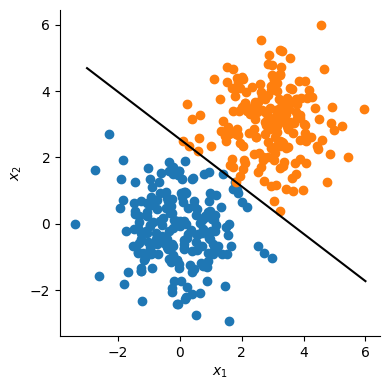
\includegraphics[scale=0.8, max width=\linewidth]{./fig/local-learning-rule/logistic-regression-perceptron/cell017.png}
	\caption{cell017.png}
	\label{cell017.png}
\end{figure}
\subsection{Target jump}

target jumpする場合の最適制御 \cite{Li2018-qt}. 状態にtarget位置も含むモデルであればtarget位置をずらせばよいが,ここでは自己位置をずらしtargetとの相対位置を変化させることでtarget jumpを実現する.
\lstinputlisting[language=julia]{./text/motor-learning/infinite-horizon-ofc/019.jl}
\lstinputlisting[language=julia]{./text/motor-learning/infinite-horizon-ofc/020.jl}
\lstinputlisting[language=julia]{./text/motor-learning/infinite-horizon-ofc/021.jl}
\lstinputlisting[language=julia]{./text/motor-learning/infinite-horizon-ofc/022.jl}
\lstinputlisting[language=julia]{./text/motor-learning/infinite-horizon-ofc/023.jl}
\begin{figure}[ht]
	\centering
	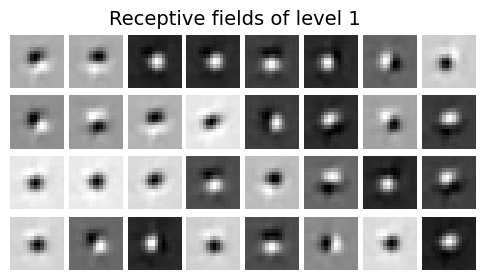
\includegraphics[scale=0.8, max width=\linewidth]{./fig/energy-based-model/predictive-coding/cell023.png}
	\caption{cell023.png}
	\label{cell023.png}
\end{figure}
